\setlength{\baselineskip}{20pt}
\chapter{基于迭代局部搜索改进的拉格朗日松弛算法设计}
\label{cha:LR算法}
拉格朗日松弛算法(Lagrangian Relaxation, 以下简称``LR算法'')
是一种基于数学优化过程的启发式方法,
是求解整数规划问题的有效手段之一。
相较于精确解法(分支定界、分支切割等),
LR算法可以在短时间内获得质量较优的近似最优解;
相较于元启发式算法(遗传算法、禁忌搜索等),
LR算法提供了优化边界(上界和下界)进而可以证明解的质量。
在求解上界时,
\replaced[id=yrf]{迭代局部搜索(Iterated Local Search, ILS)算子}{迭代局部搜索(Iterated Local Search, ILS)算法}进一步强化上界质量。
ILS算\replaced[id=yrf]{子}{法}是一种提升上界质量的方法,
其特长并不是全局搜索的能力,
而是作为其他算法的嵌入过程,提升算法整体性能。
ILS是一种易于理解的元启发式方法,
但却有强大的局部搜索能力\cite{ils}。

% 考虑节点失效风险的物流网络选址
本章为第\ref{cha:model}章的模型开发了基于迭代局部搜索改进的拉格朗日松弛
(Lagrangian Relaxation and Iterated Local Search, LR-ILS)混合算法
\replaced[id=yrf]{,该算法基于标准LR算法框架并将ILS算子嵌入其中以改进上界质量。}{。
LR是算法的整体框架,ILS是嵌入算子,}\deleted[id=yrf]{因此}
第\ref{sec:LR概述}节先推导了拉格朗日松弛的基本原理,
第\ref{sec:LR框架}节介绍了该算法的框架,
并详细阐述了上下界获取、乘子更新等细节,
第\ref{sec:小节4}节总结了本章的内容。
本章中涉及的代码均在作者的Github开源仓库中(地址见附录A),
此外本文附录A提供了全部代码,供有需要的读者下载。

\section{LR算法原理}
\label{sec:LR概述}

LR算法并非拉格朗日提出,而是后人在求解优化问题时,借鉴了拉格朗日乘数法的思路,
经过进一步概括总结,命名为拉格朗日松弛。
有关LR算法简要的发展历程如下:
LR算法可追溯至1963年Everett\cite{Everett}使用拉格朗日乘数法求解离散问题,
1973年Fisher\cite{Fisher1973}使用了该算法求解了调度问题,
Geoffrion\cite{Geoffrion1974}正式命名该算法为``拉格朗日松弛''。
LR算法已经在求解调度问题\cite{温旭红}、
选址问题\cite{yun2015}发挥了巨大作用。
本节将从一个一般的整数规划问题出发,
概述LR算法的基础原理。
更多有关LR算法的介绍及应用,
可参考Fisher\cite{Fisher2004}关于拉格朗日松弛的入门指导,
孙小玲\cite{孙小玲}有关整数规划著作中关于拉格朗日对偶理论的推导,
以及优化百科全书\cite{Hearn2009}的中关于拉格朗日松弛及拉格朗日对偶的概述。

给定一个待求解的整数规划问题P,形式如下:
$$
Z = \min c x  \quad
$$
\begin{equation}
    \begin{aligned}
        \text { s.t. }  & A x =b\\
         & D x \leq e \\
         & x \geq 0 \text { and integral }
    \end{aligned}
\end{equation}


松弛P的整数约束,得到的线性松弛问题定义为LP。
其中,$A$是$m$行$n$列的矩阵,$x$是$n$行的向量,其他所有向量的维度与之对应。
在P问题中,第一个约束是强约束,而第二个约束是弱约束。
为了处理强约束,使得问题容易求解,LR算法松弛了第一个约束,
并将其与拉格朗日乘子$\mu$相乘后添加至目标函数中。
这种处理方法借鉴了拉格朗日乘子法求多元函数极值的思路。

定义得到的松弛后的问题为$\mathrm{LR_u}$,
其中,$u=\{u_1,u_2,...u_m\}$是拉格朗日乘子:
\begin{equation}
\begin{aligned}
Z_D(u)=        & \min c x + u(Ax-b) \\
\text { s.t. } & D x \leq e \\
               & x \geq 0 \text { and integral }
\end{aligned}
\end{equation}

那么,一定有$Z_D(u) \le Z$。证明如下:
已知P问题的可行解一定是$\mathrm{LR_u}$问题的可行解。
由于$\mathrm{LR_u}$相较于P问题松弛了约束,因此可行域扩大。
令$x^*$是$P$问题的最优解,那么$x^*$未必是$\mathrm{LR_u}$的最优解
(在$\mathrm{LR_u}$的可行域内,
但不在P的可行域内,
可能存在比$x^*$更优的、
使得$\mathrm{LR_u}$目标函数值更小的解)。
因此,有$Z_D(u) \le cx^*+u(Ax^*-b)$。
当$x=x^*$时,有$Ax^*=b$,即$Ax^*-b=0$。
那么$Z_D(u) \le cx^* = Z$,证毕。

如果$Ax=b$为不等形式,则通过控制$u$的正负仍可以满足上述不等性质。
当$Ax\le b$,则令$u\ge 0$,有$Z_D(u) \le cx^* + u(Ax^*-b)=Z$。
反之同理,当$Ax \ge b$,则令$u \le 0$。

在特定的$u$的取值下,$Z_D(u)$等于$Z$。
如何给$u$取值,使得$Z_D(u)$的值尽可能大、尽可能接近$Z$的问题就变成了一个和$u$相关的问题。
该问题成为拉格朗日对偶问题D,即:
\begin{equation}
Z_D = \max _u Z_D(u)
\end{equation}
该问题的决策变量是$u$,目标函数是尽可能最大化$Z_D(u)$的值,
由于$Z_D(u)$不可能超过$Z$的值,
因此求$Z_D$的过程就是在不断调整$u$的值,使$Z_D(u)$的值逼近$Z$过程。
当前,D问题是一个抽象的形式,采用如下方法重构该问题。

假设拉格朗日松弛$\mathrm{LR_u}$的可行解集
$X=\{x|Dx\le e ,x\ge 0 \text{ and integer}\}$是有限集,
则我们可以令$X=\{x^t,t=1,...,T\}$,令$w = Z_D(u)$。
$Z_D(u)$是最小化$c x + u(Ax-b)$,
那么$Z_D(u)$一定小于等于$\mathrm{LR_u}$的任意一个可行解$x^t$带入该表达式的值,即
$Z_D(u) = w \le cx^t + u(Ax^t-b)$,
当$x^t$是$\mathrm{LR_u}$问题的最优解时等号成立。
因此,D问题重构为$\mathrm{\bar{D}}$:
\begin{equation}
\begin{aligned}
Z_D&=\quad {\rm{max}}\,w\\
\text{s.t.}\quad w &\le cx^t + u(Ax^t-b),t=1,...,T\\
\end{aligned}
\end{equation}

问题$\mathrm{\bar{D}}$的线性对偶$\mathrm{\bar{P}}$的形式如下:
\begin{equation}
\begin{aligned}
  Z_{P}= & \min \sum_{t=1}^{T} \lambda_{t} c x^{t} \\
  \text { s.t. } & \sum_{t=1}^{T} \lambda_{t} A x^{t}=b \\
  & \sum_{t=1}^{T} \lambda_{t}=1 \\
  & \lambda_{t} \geq 0, t=1, \ldots, T
\end{aligned}
  % \tag{$\mathrm{\bar{P}}$}
\end{equation}

显然$\mathrm{\bar{P}}$不是P的线性松弛,
因此$\mathrm{\bar{P}}$和LP并不是等价问题。
由于$x^t$是$\mathrm{LR_u}$的可行解,
则$x^t$是一定满足约束$Dx \le e$。
在所有满足$Dx \le e$的解中,
一定存在某个解满足$Ax=b$。
因此,当$\lambda_t$是整数时,
$\mathrm{\bar{P}}$等价于P。

问题$\mathrm{\bar{D}}$表明,
$Z_D(u)$是一系列线性函数的值的下限。
为可视化理解该过程,假设$x$的维度为1,$T$的值取4,
即$\mathrm{LR_u}$有4个可行解。
$Z_D(u)$随$u$变化如图\ref{fig:lag}所示,
\added[id=yrf]{该图源自文献\cite{Fisher2004}}。
图中加粗的黑线的表示$Z_D(u)$的取值,
表示在每个$u$固定的情况下所有线性表达的最小值。
注意图中$x^t$是已知的常数。
在这个简单例子中,$u$的线性组合是一条直线,在一般情况下是多维空间的超平面,
上述$Z_D(u)$取值操作相当于求下包络面(线)。
由此可知,$Z_D(u)$是连续且凹的(参考国际定义)但不可微的。
求$Z_D(u)$的最大值等价于求不可微的优化问题,
本文采用了次梯度法进行乘子更新,这是一种经典的乘子更新的方法。
\begin{figure}[ht] % use float package if you want it here
%\setlength{\abovecaptionskip}{-0.2cm} %调整图片caption与正文之间的间距,table同理。可自己调整。
\setlength{\belowcaptionskip}{-0.5cm} 
  \centering
  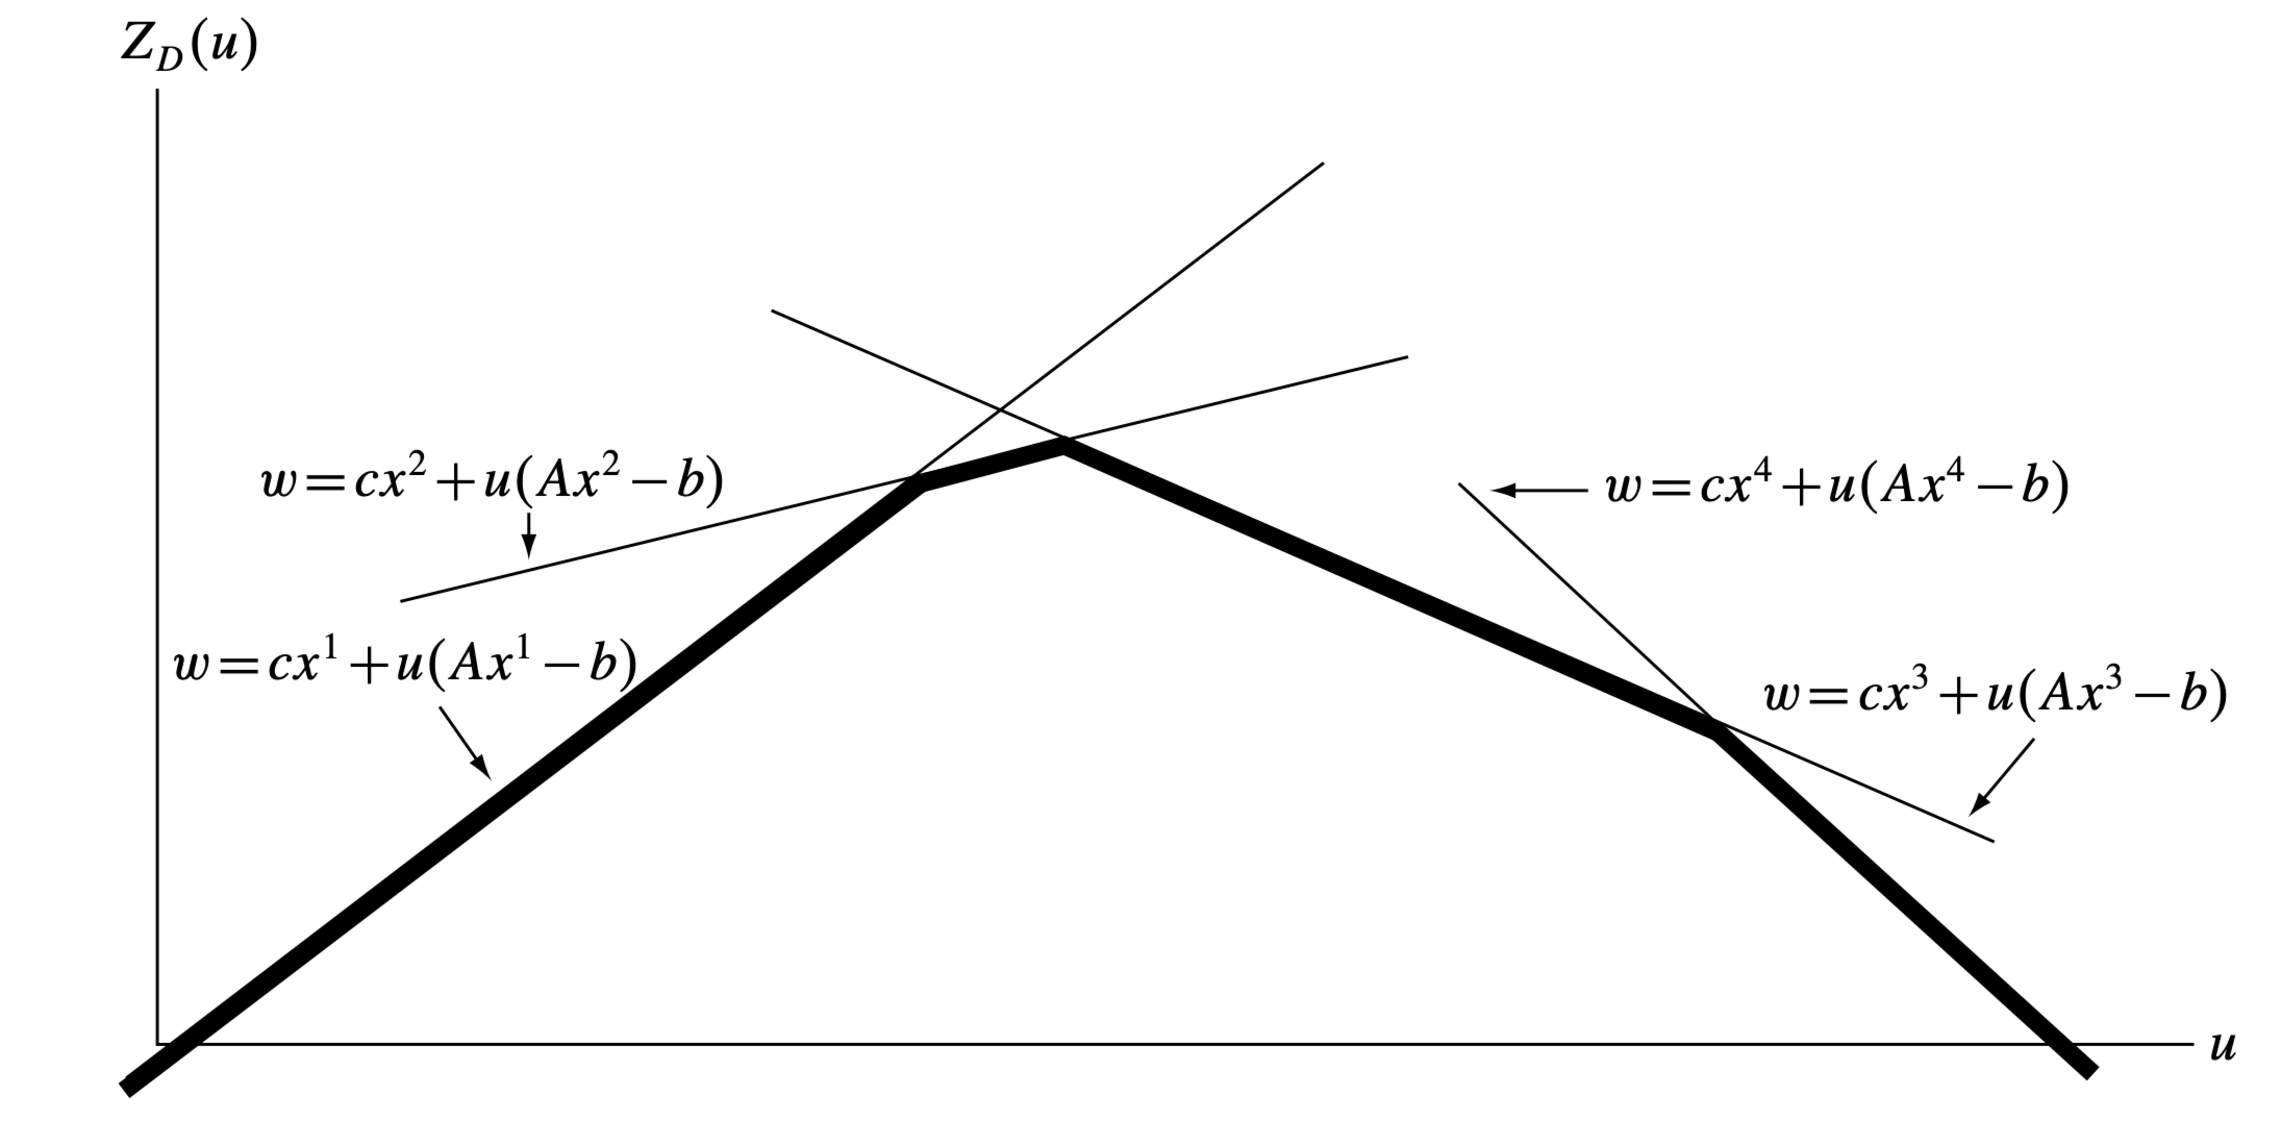
\includegraphics[width=0.9\textwidth]{figures/lag.pdf}
  \caption{$Z_D(u)$随$u$的变化(图中加粗黑线)\cite{Fisher2004} \\Fig~\ref{fig:lag}~ The value of $Z_D(u)$ as a function of $u$ \cite{Fisher2004}}
  \label{fig:lag}
\end{figure}

给定$u$的初始值$u_0$,后续乘子第$k$次迭代的值为$u^k$,迭代公式如下:
\begin{equation}
u^{k+1} = u^{k} + t_k(Ax^k-b) \label{eq:updlagmul}
\end{equation}

其中,其中$x^k$是$\mathrm{LR_{u^k}}$的最优解,
$t_k$是一个正数,称为迭代步长。
括号内的项$Ax^k-b$称作迭代方向。
Geoffrion\cite{Geoffrion1974}证明了当$t_k \rightarrow 0$
且$\sum_{i=0}^kt_i  \rightarrow \infty$时,$Z_D(u^k)  \rightarrow Z_D$。
常用的迭代步长公式如下:
\begin{equation}
   t_k = \frac{\alpha_k(Z^*-Z_D(u^k))} {||Ax^k-b||^2} 
\end{equation}

其中,$\alpha_k$是一个$(0,2]$之间的标量,$Z^*$是$Z_D$的上界,
通常由启发式获得。
$\alpha_k$的初始值一般设置为2,
当一定迭代次数后,$Z_D(u)$的值仍不能得到提升,则$\alpha_k$的值减半。

采用上述的次梯度法,不断迭代$u^k$的值,然后求解$Z_D(u^k)$,
使得松弛问题的目标函数值不断接近原问题的最优值。
需注意,由于松弛了P问题的约束,因此$Z_D(u^k)$的解对于P问题来说往往是不可行的。
通常采用启发式算法对$Z_D(u^k)$的解的进行修正,以获得P问题的可行解。

至此,本节推导了LR算法的原理。
第\ref{sec:LR框架}节将根据该原理,
为考虑节点失效风险的物流网络选址模型设计LR-ILS算法框架。

\section{算法设计}
\label{sec:LR框架}
本节将介绍采用LR-ILS算法求解考虑节点失效风险的物流网络选址模型的框架,
根据\ref{sec:LR概述}节所述,
LR算法主要包括获取下界(求解松弛模型)、获取上界、更新乘子等步骤。
注意,第\ref{sec:线性化}节中针对原模型进行了线性化处理,
所有推导内容均基于模型的线性化版本。
本节的LR-ILS算法框架参考了Snyder\cite{Snyder2005},
Yun等人\cite{yun2015, YUN2020}的文章,
以及Daskin\cite{Daskin书}使用LR关于求解UFL的方法。

为了便于理解,图\ref{fig:lr_frame}直观展示了LR-ILS的迭代流程,
图\ref{fig:lr_pseudo}提供了实现该算法的伪代码。
如图\ref{fig:lr_pseudo}所示,
在设计-ILS算法之前,需要先构造原问题M的松弛问题RM,
第\ref{subsec:约束松弛}节介绍了如何松弛问题M得到RM以及选取约束进行松弛的方法。
初始化已知最佳上界$ub^*$为正无穷,
最佳选址方案$Y^*$为空,
乘子初始化方法见第\ref{subsec:乘子更新}节。
LR-ILS算法迭代优化,
每次迭代使用精确方法获得下界(第\ref{subsec:下界获取}节),
根据下界解的选址方案构造启发式以获取上界可行解$ub$(第\ref{subsec:上界获取}节),
当上界解$ub$优于$ub^*$时,
则更新$ub^*$。
每次迭代中,LR-ILS算法使用次梯度法更新乘子,
第\ref{subsec:乘子更新}节介绍了乘子更新的方法。
当ILS条件被触发时,
ILS算法对当前解进行改进(第\ref{subsec:上界改进}节)。
若算法满足第\ref{subsec:停止条件}节的任意条件之一时,则退出迭代。
% 插入伪代码PDF代码
\begin{figure}[!ht] % use float package if you want it here
\setlength{\belowcaptionskip}{-0.5cm} 
  \centering
  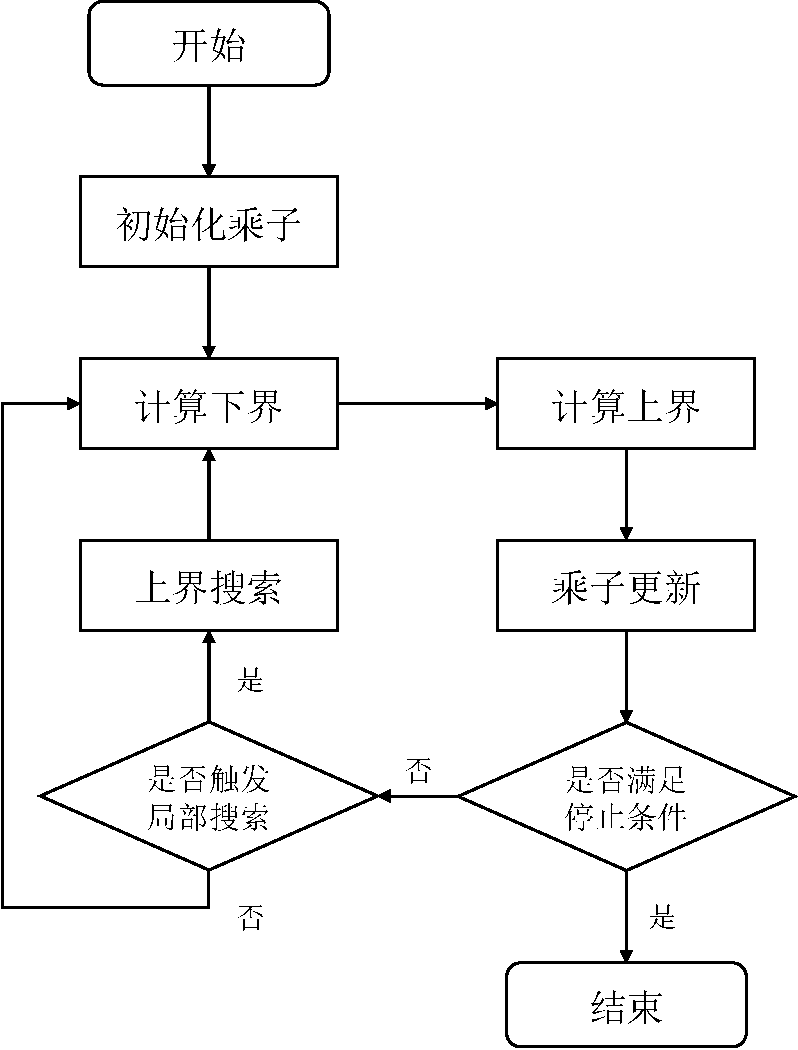
\includegraphics[width=0.5\textwidth]{figures/lr_frame.pdf}
  \caption{LR-ILS流程图\\Fig~\ref{fig:lr_frame}~ Flow chart for LR-ILS}
  \label{fig:lr_frame}
  \vspace{2ex}
\end{figure}

\begin{figure}[!ht]
    \centering
    \setlength{\belowcaptionskip}{-0.5cm} 
    \fbox{   
        \small
        \parbox[c]{0.8\textwidth}{
            \begin{algorithmic}[1] %每行显示行号
                \kaishu
                \Require 原模型M, 松弛模型RM  \Comment{ 参见第\ref{subsec:约束松弛}节}
                \State $\mu$ := 初始化乘子()  \Comment{ 参见第\ref{subsec:乘子更新}节}
                \State $ub^*$ := $+\infty$  
                \State $Y^*$ := $\emptyset$ 
                \Repeat
                    \State 下界$lb$, 选址方案$Y$ := 下界算法(RM($\mu$)) \Comment{参见第\ref{subsec:下界获取}节}
                    \State 上界$ub$ := 上界算法(M($Y$)) \Comment{ 参见第\ref{subsec:上界获取}节}
                    \If {$ub < ub^*$}                        %条件语句
                        \State $ub^*$ := $ub$
                        \State $Y^*$ := $Y$
                    \EndIf
                    
                    \State $\mu$ := 更新乘子($\mu$, $lb$, $ub^*$) \Comment{ 参见第\ref{subsec:乘子更新}节}
                    \If {ILS条件触发}                        %条件语句
                        \State $ub^*$ := ILS($ub^*$) \Comment{ 参见第\ref{subsec:上界改进}节}
                    \EndIf
                \Until{满足终止条件} \Comment{ 参见第\ref{subsec:停止条件}节}
                
                \State \textbf{return} $ub^*, Y^*$
            \end{algorithmic}
        }
    }
\caption{LR-ILS算法伪代码\\
    Fig~\ref{fig:lr_pseudo}~ Pseudocode for LR-ILS}
\label{fig:lr_pseudo}
\end{figure}



\subsection{约束松弛}
\label{subsec:约束松弛}
一般情况下,松弛不同的约束产生的效果不同,选取特定的约束进行松弛可加速求解过程。
Fisher\cite{Fisher2004}提出了两个选取松弛约束的准则:下(上)界的质量以及获得下(上)界所需计算量。
这两个准则是相互矛盾的,获得更高质量的界需要更多的计算量,较少的计算量生成的解的质量不佳。
因此,不同学者使用拉格朗日松弛求解选址问题时,构造松弛问题的方法也不尽相同,以权衡求解时长与求解质量。
Daskin\cite{Daskin书}使用拉格朗日求解UFL问题中松弛了关于所有客户都必须由某一个设施服务的约束,对应本文的约束(\ref{eq:st_assign2open})。
Snyder等人\cite{Snyder2005}求解RUFL问题松弛了每个客户的每一级都需要指派一个备用设施的约束,对应本文的约束(\ref{eq:st_trytimes})。
Yun等人\cite{YUN2020}松弛了已建成的设施才能成为客户的某一级的实体设施的约束,对应本文的约束(\ref{eq:st_assign2open})。

本文采用了Yun等人\cite{YUN2020}的松弛方法,松弛约束(\ref{eq:st_assign2open})。
使用该方法获得的松弛问题具有可继续拆分的特殊结构,利用此特性可以加快获取下界的过程。
第\ref{subsec:下界获取}节介绍了松弛问题的可拆分的特性以及获取下界的方法。

\subsection{下界获取}
\label{subsec:下界获取}
令原始模型为M,
设拉格朗日乘子$\mu = \{ \mu_{ij}\ge 0 | \forall i \in I , j \in J\}$,并将松弛的约束(\ref{eq:st_assign2open})与乘子相乘后与目标函数(\ref{eq:l_obj_model})相加,得到拉格朗日对偶问题的目标函数:
\begin{equation}
\begin{split}
\max_{\mu}\min_{x,y,w} C_D &= \sum_{j\in J}f_jy_j \\
&+ \sum_{i\in I}\lambda_i \sum_{k\in J_{ij}^+}\sum_{j\in \bar{J}} c_{kj} w_{ikj} \\
&+\sum_{i\in I}\sum_{j\in J}\mu_{ij}\left(\sum_{k\in J_{ij}^+}x_{ikj} -y_j \right)  
\end{split}
\end{equation}
整理可得,
\begin{equation}
\begin{split}
  \max_{\mu}\min_{x,y,w} C_D &= \sum_{j\in J} (f_j - \sum_{i\in I} \mu_{ij}) y_j \\
&+ \sum_{i\in I} \sum_{j\in J} \sum_{k\in J_{ij}^+} (\lambda_i c_{kj} w_{ikj} + \mu_{ij} x_{ikj}) \\
&+ \sum_{i\in I} \sum_{k\in J_{ij_0}^+}\lambda_i c_{kj_0} w_{ikj_0}  
\end{split}
\label{lag_obj}
\end{equation}
固定一组$\mu$的值,得到的松弛模型RM($\mu$)如下,为了方便阅读,本节给出了RM($\mu$)的约束,
这些约束与第\ref{sec:线性化}节中的线性约束是一致的。
\begin{equation}
\begin{split}
\min_{x,y,w} C_D(\mu) &= \sum_{j\in J} (f_j - \sum_{i\in I} \mu_{ij}) y_j \\
&+ \sum_{i\in I} \sum_{j\in J} \sum_{k\in J_{ij}^+} (\lambda_i c_{kj} w_{ikj} + \mu_{ij} x_{ikj}) 
+ \sum_{i\in I} \sum_{k\in J_{ij_0}^+}\lambda_i c_{kj_0} w_{ikj_0}  
\end{split}
\label{eq:rm_obj}
\end{equation}
\textit{s.t.}
\begin{gather}
\sum_{j\in J_{ii}^-}x_{iij} = \sum_{j\in J_{i{j_{0}}}^+} x_{ijj_0} = 1, \forall i \in I  \label{eq:rm_flow}\\
\sum_{k\in J_{ij}^-} x_{ijk} = \sum_{k\in J_{ij}^+} x_{ikj}, \forall i \in I, j \in J    \\
p_{iij} = x_{iij}, \forall i\in I, j\in J_{ii}^- \\
q_j\sum_{k\in J_{ij}^+} w_{ikj}= p_{ijj'}, \forall i \in I, j \in J, j'\in J_{ij}^- \\
\sum_{j\in J\cup\{i\}} \sum_{k\in J_{ij}^-} x_{ijk} \le R, \forall i\in I \\
w_{ijk} \le p_{ijk}, \forall i \in I, j \in J, j'\in J_{ij}^- \\
w_{ijk} \le x_{ijk}, \forall i \in I, j \in J, j'\in J_{ij}^- \\
w_{ijk} \ge p_{ijk} + x_{ijk} - 1, \forall i \in I, j \in J \cup \{i\}, j'\in J_{ij}^-
\end{gather}
\begin{equation}
0 \le w_{ijj'r} \le 1, \forall i \in I, j \in J, j'\in J_{ij}^- 
\end{equation}
\begin{equation}
x_{ijk} \in \{0,1\}, \forall i \in I, j \in J\cup \{i\}, k\in J_{ij}^-
\end{equation}
\begin{equation}
0 \le p_{ijk} \le 1, \forall i \in I, j \in J\cup \{i\}, k\in J_{ij}^- \label{eq:rm_p}
\end{equation}
\begin{equation}
y_{j} \in\{0,1\}, \forall j \in {J} \label{eq:rm_y}
\end{equation}

对于给定的任意$\mu$的值,RM($\mu$)的最优解一定是M的下界,相关证明见\ref{sec:LR概述}节。
根据目标函数(\ref{eq:rm_obj})的结构,松弛模型RM($\mu$)可拆分成两组子模型RM($\mu$)$_{sub1}$和RM($\mu$)$_{sub2}$。
其中,RM($\mu$)$_{sub1}$如下,
\begin{equation}
\min_{y} \sum_{j\in J} (f_j  - \sum_{i\in I}\mu_{ij}) y_j
\end{equation}
\textit{s.t.}
\begin{center}
   约束(\ref{eq:rm_y})
\end{center}
RM($\mu$)$_{sub2}$如下,
\begin{equation}
\max_{\mu}\min_{x,w} 
\sum_{i\in I} \sum_{j\in J} \sum_{k\in J_{ij}^+} (\lambda_i c_{kj} w_{ikj} + \mu_{ij} x_{ikj}) 
+ \sum_{i\in I} \sum_{k\in J_{ij_0}^+}\lambda_i c_{kj_0} w_{ikj_0}
\label{eq:rm2_obj}
\end{equation}
\textit{s.t.}
\begin{center}
   约束(\ref{eq:rm_flow}) - 约束(\ref{eq:rm_p})
\end{center}

在给定任意一组$\mu$的值的情况下,RM($\mu$)$_{sub1}$将变得十分容易求解,即给定一个最小化问题$\min_{y} \sum_{j\in J} (f_j  - \sum_{i\in I}\mu_{ij}) y_j$,其中$y_j,\forall j \in J$是0-1变量。
显然,
当$f_j - \sum_{i\in I}\mu_{ij} \ge 0 $时,$y_j=0$;
当$f_j - \sum_{i\in I}\mu_{ij} < 0 $时,$y_j=1$。

在给定任意一组$\mu$的值的情况下,RM($\mu$)$_{sub2}$还可进一步拆分成$|I|$个独立模型,
每个子模型RM($\mu$)$_{sub2}^i, \forall i \in I$是试错序列问题更一般的形式,
该问题的具体表述见第\ref{subsec:subprob}节。
RM($\mu$)$_{sub2}^i$与第\ref{subsec:subprob}节中介绍的问题的不同之处在于RM($\mu$)$_{sub2}^i$的目标函数不仅计算了期望成本,还计算了关于$\mu$的项。
不妨将$\mu_{ij}, \forall i \in I , j \in J$看作是客户$i$访问节点$j$的固定访问成本,
那么,RM($\mu$)$_{sub2}^i$可理解为从$i$点出发,
寻找一条到$j_0$的期望成本与固定访问成本最小的路径,
并且该路径经过的虚拟节点和实体节点总数不得大于$R$个。

本节已经给出了RM($\mu$)$_{sub2}$的线性混合整数规划模型,
使用上述的拆分方法固定$i\in I$的值即可获得RM($\mu$)$_{sub2}^i$,
然后可使用求解器求解RM($\mu$)$_{sub2}^i$。
当$\mu=0$时,
RM($\mu$)$_{sub2}^i$等价于第\ref{subsec:subprob}节中介绍的试错序列问题。
RM($\mu$)$_{sub2}^i$实质上是一个广义的最短路问题,
由于该问题是NP-hard问题,使用精确求解方法的计算时间较长,
而LR算法会多次迭代并反复调用求解该问题的方法,
因此本节给出两种快速求解RM($\mu$)$_{sub2}^i$的启发式算法以及一个精确方法。
启发式方法生成一个近似解,
精确方法在这个近似解的基础上进行改进,
可加快求解速度并获取下界的精确值。

(1){\textbf{插入启发式}}

已知客户$i$一定会从点$i$出发最终前往虚拟节点$j_0$,
因此可初始化一个从客户$i$到虚拟设施$j_0$的初始序列$s_i$。
在该方法中,$s_i$的期望成本与固定访问成本之和,即目标函数(\ref{eq:rm2_obj}),
记作$C_{lb}(s_i)$。
定义$s_i$中连续两点之间的位置集合为$P(s_i)$。
插入启发式算法的步骤如下:
\begin{enumerate}[leftmargin=0pt,itemindent=3.5\ccwd,nosep]
  \item[Step 0] 初始化序列$s_i:=[i,j_0]$, 计算$C_{lb}(s_i)$。
  \item[Step 1] 向$s_i$中每个位置$\rho \in P(s_i)$添加节点$j \in J$,并计算成本$C_{lb}^{\rho j}(s_i)$。
  \item[Step 2] 计算$\Delta_{\rho j} = C_{lb}(s_i) - C_{lb}^{\rho j}(s_i)$。
  \item[Step 3] 若所有$\Delta_{\rho j}<0$,则结束;否则将$\Delta_{\rho j}$最大值对应的节点$j^*$插入$s_i$的$p^*$位置,
  更新$s_i$,$P(s_i)$,$C_{lb}(s_i)$以及令$J:=J\backslash\{j^*\}$。
  \item[Step 4] 若$J=\emptyset$或$|s_i|=R+1$,则结束,否则重复Step 1-4。
\end{enumerate}

插入启发式从一个仅包含客户和虚拟节点的完整的初始序列出发,
因此初始序列的总成本等于惩罚成本。
每次插入实体节点之前,
评估每个节点插入每个位置之后得到的结果,
然后将实体节点插入序列中当前阶段的最佳位置,
使得总成本快速下降,直至不能插入任何节点。

(2){\textbf{构造启发式}}

已知客户$i$一定会从点$i$出发前往虚拟节点$j_0$。
构造启发式仅考虑每一阶段的最优,
向序列末尾逐个增加节点,
具体步骤如下:
\begin{enumerate}[leftmargin=0pt,itemindent=3.5\ccwd,nosep]
  \item[Step 0] 初始化序列$s_i:=[i]$, 令$C_{lb}(s_i)=0$。
  \item[Step 1] 计算所有点$j \in \bar{J}$添加至$s_i$末尾的增量成本$\Delta_{j} = C_{lb}(s_i+\{j\}) - C_{lb}(s_i)$。
  \item[Step 2] 令$j^* = \arg \min \Delta_{j}$,更新$s_i:=[s_i, j^*]$和$C_{lb}(s_i)$,$J:=J\backslash\{j^*\}$。
  \item[Step 3] 若$j^*=j_0$,则结束;若$|s_i|=R$,则$s_i:=[s_i, j_0]$,计算$C_{lb}(s_i)$并结束,否则重复Step 1-3。
\end{enumerate}

构造启发式从一个仅含客户的不完整路径出发,
每次向路径的末尾增加一个节点。
每次增加的过程都将增量成本最小的客户放在末尾,
直至添加了虚拟节点(构成了完整路径)或不再能添加节点(此时在末尾补充一个虚拟节点构成一个完整路径)。

上述两种算法均基于贪心算法,
插入启发式算法先接受高昂成本,
再插入节点以降低总成本。
插入启发式类似节约算法,初始成本很高,成本随节点插入逐渐降低。
构造启发式算法从无到有,逐渐拓展路径的长度,
每次拓展将增量成本最低的节点加入路径末尾。
插入启发式算法时间复杂度等于$O(m^2n)$,
构造启发式算法时间复杂度等于$O(mn)$,
其中$m=R$是客户拥有实体节点个数的上限,
$n=|J|$是备选点的数量。

需要注意,在给定$\mu$的值的前提下,上述的两种方法仅可以在多项式时间内获得近似最优解,
而不一定可以获得最优解。
这将导致RM($\mu$)$_{sub2}$不能获得最优解。
已知只有在子问题获得最优的前提下,才能保证下界小于上界(证明见第\ref{sec:LR概述}节)。
因此,采用上述方法获得的下界很有可能在最终收敛时超过上界,使算法无法证明上界的质量。

求解最短路问题经典的精确算法包括标签算法\cite{label}、脉冲算法\cite{pulse}等。
但这些算法不能直接应用于试错序列问题,
因为这些算法解决的问题中每个点并不存在失效概率,
且总成本等于路径长度简单和。
由于上述的启发式算法可以获得一个近似最优解,
本文将上述启发式算法获得的近似最优解带入深度优先搜索算法(Deep First Search, DFS),
并设计剪枝策略以求解试错序列问题的最优解。

(3){\textbf{DFS算法}}

DFS算法的伪代码如图\ref{fig:dfs_pseudo}所示。
DFS类似于构造启发式,
从客户点出发,
每一次向下分支就将一个节点添加至路径末尾,
直至遍历完这个分支的所有可能,
再选择该分支的某个分支继续遍历,
如此递归直至遍历完问题的所有可能。
对于该问题来说,递归的最大深度是有限的,
判定某个路径$s_i$是否到达最大深度的准则有三个: 
(1) $\bar{J} = \emptyset$; 
(2) $|s_i| = R$, 此时$s_i$只能以$j_0$结尾;
(3) $s_i$的已经以$j_0$结尾。
当搜索满足上述三种情况之一时,不再继续分支(到达叶子节点)。
然后计算路径成本$C_{ib}({s_i})$。
当$C_{ib}({s_i})$小于已知最优成本$C_{ib}({s_i^*})$,
则更新已知最优路径和已知最优成本。
DFS分支的过程采用了递归调用,
当搜索未达到最大搜索深度时,
继续向下分支的过程中,保存当前的父节点并在遍历完子节点及所有分支后恢复。
分支过程中,若当前路径的成本$C_{ib}({s_i+\{j\}})$大于已知最优成本$C_{ib}({s_i^*})$时,
则不再继续分支(剪枝)。

% \begin{figure}[hbt] % use float package if you want it here
%   %\setlength{\abovecaptionskip}{-0.2cm} %调整图片caption与正文之间的间距,table同理。可自己调整。
%   \setlength{\belowcaptionskip}{-0.5cm} 
%     \centering
%     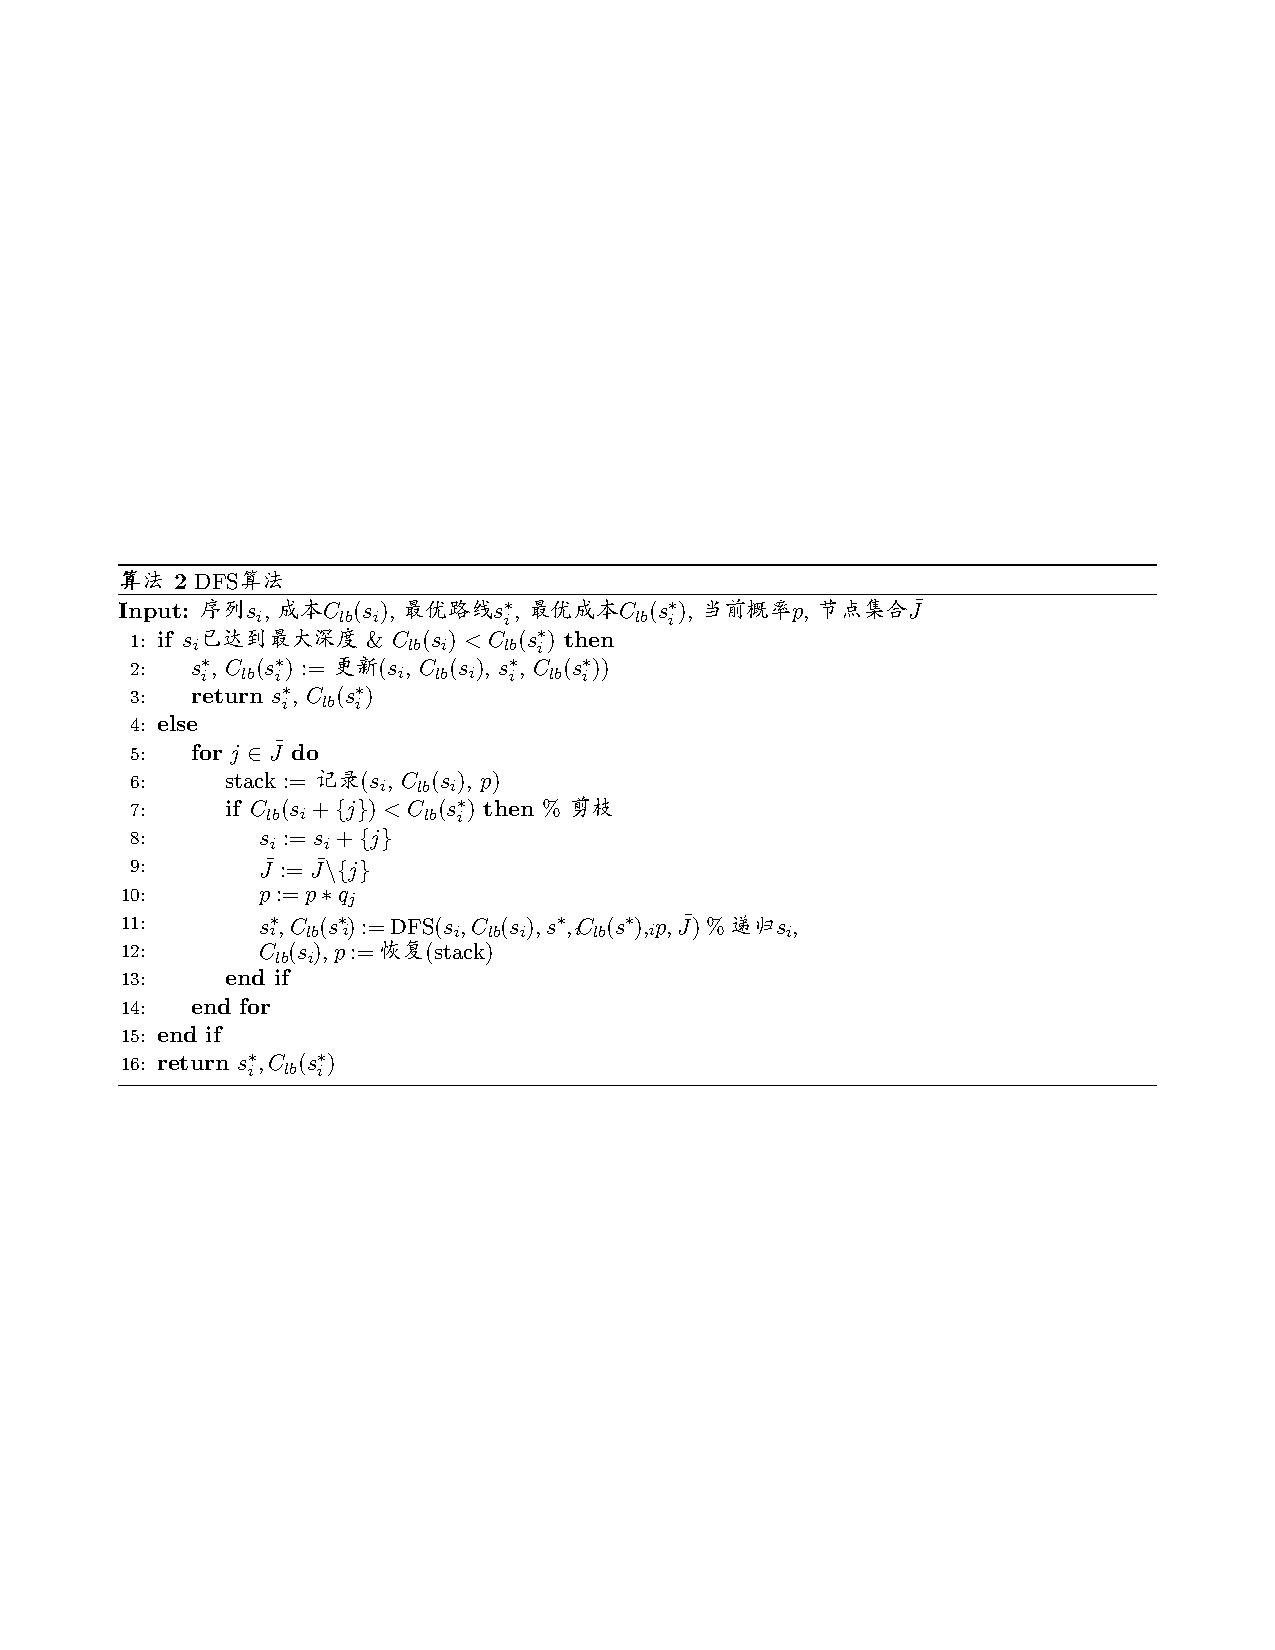
\includegraphics[width=\textwidth]{figures/dfs.pdf}
%     \caption{DFS算法伪代码。\\Fig~\ref{fig:dfs_pseudo}~ Pseudocode for DFS.}
%     \label{fig:dfs_pseudo}
% \end{figure}

\begin{figure}[htb]
    \centering
    \setlength{\belowcaptionskip}{-0.5cm} 
    \fbox{   
        \small
        \parbox[c]{0.9\textwidth}{
             \begin{algorithmic}[1] %每行显示行号
             \kaishu
                \Require 序列$s_i$, 成本$C_{lb}(s_i)$, 最优路线$s_i^*$, 最优成本$C_{lb}(s_i^*)$, 当前概率$p$, 节点集合$\bar{J}$
                % \Ensure 最优上界$ub^*$
                \If {$s_i$已达到最大深度~\&~$C_{lb}(s_i)<C_{lb}(s_i^*)$}                       %条件语句
                    \State $s_i^*$, $C_{lb}(s_i^*)$ := 更新($s_i$, $C_{lb}(s_i)$, $s_i^*$, $C_{lb}(s_i^*)$)
                    \State \textbf{return} $s_i^*$, $C_{lb}(s_i^*)$
                \Else
                    \For {$j \in \bar{J}$} 
                        \State stack := 记录($s_i$, $C_{lb}(s_i)$, $p$)
                        \If {$C_{lb}(s_i + \{j\})<C_{lb}(s_i^*)$} \% 剪枝
                            \State $s_i:=s_i + \{j\}$
                            % \State $C_{lb}(s_i)$ :=$C_{lb}(s_i + \{j\})$
                            \State $\bar{J} :=\bar{J} \backslash \{j\}$
                            \State $p: = p * q_j$
                            \State $s_i^*$, $C_{lb}(s_i^*)$ := DFS($s_i$, $C_{lb}(s_i)$, $s_i^*$, $C_{lb}(s_i^*)$, $p$, $\bar{J}$) \quad \% 递归
                            \State $s_i$, $C_{lb}(s_i)$, $p$ := 恢复(stack)
                        \EndIf  
                    \EndFor
                \EndIf
                \State \textbf{return} $s_i^*, C_{lb}(s_i^*)$
            \end{algorithmic}
        }
    }
\caption{DFS算法伪代码\\Fig~\ref{fig:dfs_pseudo}~ Pseudocode for DFS}
    \label{fig:dfs_pseudo}
\end{figure}


理论上,DFS可以求解任何最短路问题,
但是该算法并不是多项式时间算法,因此并不能保证计算时长在合理范围内。
本文可以采用DFS算法是因为搜索深度和客户的最大试错次数$R$正相关,
计算时间随搜索深度指数级增长,
但通常$R$的值并不会很大,
这使得DFS方案可行。
其次,上述的两个启发式方法可以获得近似解,
利用这个近似解可以在搜索过程中剪枝,
避免遍历所有情况。
最后,所有的成本均为非负值,即所有弧的权重为非负值,
这使得一条不完整路径$s_i$(不一定以$j_0$结尾)的产生的成本$C_{lb}(s_i)$
一定小于等于$s_i$被节点$\{j\}$拓展的路径的成本$C_{lb}(s_i+\{j\})$,
即到达子节点产生的费用一定大于等于父节点的费用。

综上,求解下界问题相当于求解一个最短路问题,
由于该问题是NP-hard问题,
本小节给出了两种多项式时间的启发式算法以获得近似最优解,
以近似最优解为已知最优解,
使用了DFS算法进行剪枝搜索以获得下界最优解。
此外,本小节给出了求解下界的数学规划模型,
亦可使用求解器对下界进行求解。

\subsection{上界获取}
\label{subsec:上界获取}
子问题的RM($\mu$)$_{sub1}$的解给出了选址方案$J^*$,
令选址方案对应的选址决策变量$y_j=1,\forall j\in J^*$
以及选址方案以外的选址决策变量$y_j=0,\forall j\in J \wedge j\notin J^*$,
作为约束条件加入原模型M中,
使用精确算法求解该模型,即可获得原模型的上界。
上界值等于建设节点的固定成本再加上客户的期望运输成本之和。
在已知选址方案$J^*$的情况下,
建设节点的固定成本等于被选中的候选节点的固定成本$f_j$的简单和。
已知选址方案$J^*$,求解客户的期望运输成本之和,
完全等价于第\ref{subsec:subprob}节介绍的试错序列问题,
即令拉格朗日乘子等于0。

然而,客户试错序列问题是一个NP-hard问题(第\ref{subsec:subprob}节给出了证明),
求解该问题的启发式算法以及精确方法已在第\ref{subsec:下界获取}节中介绍。
相较于下界,求解上界的过程较为简单:
首先,下界问题中所有的候选节点都可以被使用,
而在求解上界的过程只能使用已经建成的节点,问题规模缩小。
其次,下界问题中所有节点的都存在固定成本(拉格朗日乘子),
而上界问题中不存在固定成本。

由于本文考虑的是无容量限制的问题,
因此在给定选址方案后,模型可拆分成$|I|$个子问题,
这些子问题的最优解之和等于上界最优解,
每个子问题等价于试错序列问题也等价于RM$(\mu)_{sub2}^i$,
因此上界完全可以使用第\ref{subsec:下界获取}节中介绍的算法,
但为了加速获得每个客户的试错序列、获得高质量上界,
本节介绍了一种Dijkstra的变种算法,可以在多项式时间内求解上界。
注意该算法仅能快获得一个近似最优解,
并仅在不考虑访问节点固定成本(求解上界无拉格朗日乘子)的情况下表现良好。
类似Dijkstra原始版本,采用永久标号法的步骤如下:

\begin{enumerate}[leftmargin=0pt,itemindent=3.5\ccwd,nosep]
  \item[Step 0] 初始化每个节点的权重为$\infty$,到达每个节点的概率$p_j$为1,每个点的状态为未标记,设置客户为起点,每个节点的追踪标记等于客户。
  \item[Step 1] 从起点出发,计算到达所有未标记节点所需的成本,如果到达当前未标记节点的所需费用小于节点的权重,则更新该节点的权重。
  \item[Step 2] 在所有未标记节点中,找到权重最小的节点,将其设为起点,更新其到达概率等于上一个节点的到达概率乘以上一个节点的失效概率,更新其追踪标记为上一个起点。
  \item[Step 3] 重复Step 1-2。若当前起点为$j_0$,则结束,返回当前点的权重。
  若逆向追踪得到的路径中节点和客户总数等于$R$,则在路径最后补充一个$j_0$,计算路径成本,结束并返回路径成本。
\end{enumerate}

该算法对经典Dijkstra算法进行了修改,
在原有算法的基础上引入了到达该节点的概率,
并添加了终止规则。
算法的时间复杂度等于$O(mn)$,
其中$m$是客户最大尝试次数,
$n$是节点的个数。
该算法可以求解上界近似最优解,也可以求解下界近似最优解。
但是,求解下界解时加入了节点的固定访问成本,增加问题的复杂性,
使得这种方法求解下界的效果不佳。
在求解上界的过程中,由于不存在固定访问成本(拉格朗日乘子),
算法迭代更新虚拟设施$j_0$的权重的次数提升,
而每次更新$j_0$后,经过逆向追踪都可以获得一条更优的完整路径。
因此,求解上界的Dijkstra的变种算法并不适用于下界求解。
此外,Yun\cite{YUN2020}等人设计了一种辅助图方法,
基于辅助图,开发了另一种求解客户试错序列问题Dijkstra的变种算法。

回到整个拉格朗日算法框架,
获得上界的前提是子问题RM($\mu$)$_{sub1}$的解给出了选址方案$J^*$,
基于已知的选址方案可以获得质量较好的上界\cite{Daskin书,yun2015}。
本小节介绍了获取上界的方法,
根据已知的选址方案,使用Dijkstra变种算法生成每个客户的试错序列。
然而该方法对于求解下界效果不佳,但可以用来求解上界的近似最优解。
此外,求解下界的DFS方法同样适用于求解上界客户试错序列问题中,
将Dijkstra变种算法得到的解传递给DFS算法,
可在此近似解的基础上得到最优解,
该方法的详细操作见本章第\ref{subsec:下界获取}节。

\subsection{乘子更新}
\label{subsec:乘子更新}
第\ref{sec:LR概述}节介绍了LR算法常采用次梯度法进行乘子更新。
本文的算法和大多数LR算法一样\cite{Daskin书,yun2015,Snyder2005},
其算法的效率很大程度依赖乘子$\mu$的初始值。
合理的乘子初始值可以减少算法的迭代步骤,进而提升效率。
本文乘子初始值设定参考了Lim\cite{lim}的方法,
令$\mu^k=\{\mu_{ij}^k \ge 0\}$表示算法第$k$迭代时的乘子$\mu$的取值,
$\mu^0$表示乘子的初始值,其计算公式如下:

\begin{equation}
    \mu_{ij}^0 = \frac{1}{|J|}(\lambda_i c_{ij} + f_j), \forall i \in I, j\in J
\end{equation}

在第\ref{sec:LR概述}节拉格朗日松弛概述中,
公式(\ref{eq:updlagmul})展示了一般问题中拉格朗日乘子更新的迭代方法。
针对原问题M,乘子更新方法如公式(\ref{eq:updatemulti})所示,
\begin{equation}
\mu^{k+1}_{ij} = \mu^{k}_{ij} + t_k(\sum_{k\in J_{ij}^+}x_{ikj} -y_j),\forall i\in I,j\in J
\label{eq:updatemulti}
\end{equation}

其中,$t_k$表示迭代步长,计算方式如下,
\begin{equation}
t_k = \frac{\alpha_k(ub_k^* - lb_K)} {\sum_{i\in I}\sum_{j\in J}\sum_{k\in J_{ij}^+}|x_{ikj} -y_j|}
\label{eq:steplen}
\end{equation}

公式(\ref{eq:steplen})中$ub_k^*$和$lb_K$分别表示第$k$次迭代的已知最佳的上界和下界,
迭代步长系数$\alpha_k$是一个常量,
当算法连续$\kappa_{lb}$次迭代都未能使下界提升时(一般在情况下,下界会在此时产生振荡),
$\alpha_k$将除以比例因子$\theta_{lr}$,以缓解振荡。
关于公式(\ref{eq:steplen})右侧分母项,
本文参考了Yun\cite{YUN2020}关于迭代步长的设计,
修改了经典拉格朗日算法迭代步长分母取平方操作,
改用绝对值,以获得更优的收敛性。

\subsection{停止条件}
\label{subsec:停止条件}
为了在有限的时间内获得高质量的上界,
证明上界的质量,避免程序无意义的迭代,
当LR-ILS算法满足下列条件其中之一时,算法停止迭代:

\begin{enumerate}[label=(\arabic*),leftmargin=0pt,itemindent=3.5\ccwd, nosep]
    \item 迭代次数$k$大于等于最大迭代次数$\eta_{lr}$;
    \item 算法优化时长到达时间上限$\tau_{lim}$;
    \item 上下界间隙(gap)$(ub_k-lb_K)/ub_k \le \xi$;
    \item 迭代步长系数$\alpha_k <= \alpha_{min}$。
\end{enumerate}

条件(1)限制了拉格朗日算法的迭代次数,
条件(2)限制程序的运行时长,
条件(3)表明期望接受的解的优劣程度,
条件(4)避免算法后期不能提升下界的无用迭代。

\subsection{上界改进}
\label{subsec:上界改进}
上述小节\ref{subsec:约束松弛}至小节\ref{subsec:停止条件}已详细阐述了LR-ILS算法的细节,
使用上述方法可以获得可接受的结果\cite{yun2015,Daskin书,Fisher2004}。
但上述算法仍有一些缺陷:
上界解的选址方案是由下界解提供的,
下界解在算法后期收敛过程中并不能提供足够优质的选址方案,
或者下界在后期产生振荡。
为了加速算法上下界的收敛,
本节介绍的迭代ILS算法\deleted[id=yrf]{(Iterated Local Search, ILS)}对当前最佳选址方案$J^*$进行改进。


ILS算法可以作为独立的一种元启发式算法求解考虑节点失效风险的物流网络选址模型,
即在ILS每次迭代中,ILS提供选址方案,
再根据第\ref{subsec:上界获取}节获取上界的方法评估方案质量,
不断迭代直至算法连续多次迭代都不能获得更优解时结束。
但在本文中,将ILS嵌入LR迭代框架中(见图\ref{fig:lr_pseudo}),
当ILS算法被触发,会对$J^*$进行邻域搜索,
并将搜索到的更优解返回给LR,
以减少上下界之间的间隙。

本文嵌入的ILS算法的框架设计参考了Lourenço\cite{ils}等人书中内容,
该算法的伪代码如图\ref{fig:ils}所示。
ILS算法是一种基于单个解的局部搜索算法,
给定一个初始选址方案$J^*$(已知最优解),
ILS使用邻域算子搜索其邻域,
根据一定准则接受邻域中某个邻域解,
然后从这个邻域解出发继续搜索,搜索其邻域,
如此往复,迭代进行。
在搜索过程中,如果发现某个解优于已知最优解,
则用这个解替换已知最优解,并提前结束返回该解。

\begin{figure}[ht] % use float package if you want it here
%\setlength{\abovecaptionskip}{-0.2cm} %调整图片caption与正文之间的间距,table同理。可自己调整。
\setlength{\belowcaptionskip}{-0.5cm} 
  \centering
  \fbox{   
        \small
        \parbox[c]{0.9\textwidth}{
            \begin{algorithmic}[1] %每行显示行号
                \kaishu
                \Require 选址方案$J^*$
                \State 已知最佳选址方案$J^*_{best}$ := $J^*$
                \Repeat 
                    \State 邻域$\mathcal{N}(J^*)$ := 邻域算子($J^*$)
                    \State $obj_{\mathcal{N}(J^*)}$ := 目标函数($\mathcal{N}(J^*)$)
                    \If {min($obj_{\mathcal{N}(J^*)}$)$< obj_{J^*_{best}}$}
                        \State $J^*_{best}$ := $j$
                        \State \Return $J^*_{best}$
                    \Else 
                        \State $J^*$ := 接受准则($\mathcal{N}(J^*)$)
                    \EndIf
        
                \Until 终止条件满足
                \State \Return $J^*_{best}$
            \end{algorithmic}
        }
    }
  \caption{ILS算法伪代码\\Fig~\ref{fig:ils}~ Psuedocode for ILS}
  \label{fig:ils}
\end{figure} 

算法的邻域搜索过程包括三种算子\cite{sa_lp,ts_lp}:关闭、开启、交换算子。
关闭算子是指关闭$J^*$中的某个已建设节点,使得固定成本下降,运输成本上升,
以在效益背反的博弈中使得总成本降低;
开启算子是指开启$J^*$中的某个未建设节点,使得固定成本上升,运输成本下降;
交换算子是指交换$J^*$中关闭某个已建设节点并开启某个未建设的节点。

每次迭代ILS评估所有邻域解的质量,发现更优的解将返回这个解,
若没有发现更优解,则接受一个相对较差的解。
接受准则借鉴了模拟退火算法的设计思路\cite{sa},
当邻域解$j^*\in \mathcal{N}(J^*) $未改进$J^*_{best}$时,
$j^*$仍有$e^{[{obj(j^*)-obj(J^*_{best})}] / T}$的概率被接受,
其中$T$为模拟退火温度,
其初始值设定为$T_0$。
$T_0$的取值应使得ILS在$obj(j^*)/obj(J^*_{best})=\theta_{sa}$时的接受概率等于50\%,
其中$\theta_{sa}$是常数。
即在ILS算法初次迭代时,如果某个邻域解的目标函数是已知最优目标函数值$\theta_{sa}$倍时,
ILS有50\%的概率接受这个解。
温度$T$随ILS迭代次数线性减少,但不低于$T_{min}$。

当LR迭代过程中,连续$\kappa_{ub}$次未降低上界时,
ILS算法被触发。
ILS算法至多迭代$\eta_{ils}$次,
该值应设置成一个较小的数,
因为过多的搜索次数将降低算法整体的迭代效率。
此外,ILS也可以将当前迭代的邻域传递给下一次ILS触发,
相当于搜索算法的重启操作\cite{vrpdst},
重启ILS很可能产生不同的搜索过程,进而提升发现更优解的概率。

% 此外,除了在迭代过程中可以使用ILS改进上界,
% 在LR-ILS算法结束后,将最佳选址方案转为约束条件,
% 添加至原模型M中,
% 并使用求解器求解一次模型,
% 可以获得更加优质的上界,
% 以解决第\ref{subsec:上界获取}节Dijkstra变种算法不能获得最优试错序列的缺点。

\section{本章小结}
\label{sec:小节4}
本章阐述了求解考虑节点失效风险的物流网络选址模型的算法,
第\ref{subsec:约束松弛}节松弛了模型中所有客户必须分配给已建设设施的约束,
使得松弛问题可以拆分成多个子问题。
其中求解每个子问题的过程等价于一个最短路问题,
第\ref{subsec:下界获取}节采用了启发式加深度优先搜索算法求解这个子问题。
松弛模型的节提供了选址方案,
将该选址方案提供给上界问题(原模型),
求解上界的过程仍然是求解最短路问题,
第\ref{subsec:上界获取}节开发了Dijkstra变种算法,
在多项式时间内求解客户在给定选址方案的情况下的试错序列。
第\ref{subsec:乘子更新}节和
第\ref{subsec:停止条件}节阐述了拉格朗日乘子更新和停止条件。
特别地,本章的第\ref{subsec:上界改进}节给出了上界改进的方法,
介绍了一种可以嵌入拉格朗日松弛迭代中可以改进上界的ILS算法。
最后,值得一提的是,本章中所有的求解上界或下界的过程,
都可以使用求解器进行求解,
虽然求解时间随问题规模指数增长,
但提供了一种检验自设计算法有效性的方法或标准。
第\ref{cha:算法性能章}章对算法的性能进行了详细的分析,包括求解时间、求解质量等指标。
